\documentclass[titlepage=firstiscover, captions=tableheading, bibliography=totoc]{scrartcl}
\usepackage[autostyle=true,german=quotes]{csquotes}
\usepackage{scrhack}
\usepackage{caption}
\usepackage[aux]{rerunfilecheck}
\usepackage{subcaption}        
\usepackage{fontspec}
\usepackage[dvips]{graphicx}
\usepackage{floatflt,epsfig} 
    
\usepackage{polyglossia}
\setmainlanguage{german}

\usepackage[unicode]{hyperref}
\usepackage{bookmark}
\title{V27\\ Der Helium-Neon-Laser}
\author{
Miriam Simm\\
\texorpdfstring{\href{mailto:miriam.simm@tu-dortmund.de}{miriam.simm@tu-dortmund.de}\and}{,}
Katrin Bolsmann\\
\texorpdfstring{\href{mailto:katrin.bolsmann@tu-dortmund.de}{katrin.bolsmann@tu-dortmund.de}}{}
}
\date{Durchführung: 15.06.2020 \\ Abgabe: -.06.2020}
\usepackage{amsmath} 
\usepackage{amssymb} 
\usepackage{mathtools}
\usepackage[
    math-style=ISO,
    bold-style=ISO,
    sans-style=italic,
    nabla=upright,
    partial=upright,
]{unicode-math}
    
\setmathfont{Latin Modern Math}

\usepackage[
  locale=DE,
  separate-uncertainty=true, 
  per-mode=symbol-or-fraction,
]{siunitx}

\usepackage{multicol}
\setlength{\columnsep}{1pt} %space between columns 

\usepackage{booktabs}
\usepackage[x11names, table]{xcolor}
\usepackage{graphicx}
\usepackage{grffile}
\usepackage{xfrac}
\usepackage{xcolor}

\usepackage{float}
\floatplacement{figure}{h}
\floatplacement{table}{h}
\usepackage[
  section,
  below,
]{placeins}

\usepackage{expl3}
\usepackage{xparse}
\ExplSyntaxOn
\NewDocumentCommand \E {} {\symup{e}}
\ExplSyntaxOff

% Literaturverzeichnis
\usepackage[
  backend=biber,
]{biblatex}
% Quellendatenbank
\addbibresource{literatur.bib}

\usepackage[
  version=4,
  math-greek=default,
  text-greek=default,
]{mhchem}
 

\raggedcolumns

\begin{document}

\maketitle

\section{Zielsetzung}
In diesem Versuch soll mit dem Verfahren des optischen Pumpens die Energiedifferenz der Zeeman-Aufspaltung gemessen und aus dieser der Lande-Faktor des Alkalimetalls Rubidium bestimmt werden.


\section{Theorie}
Die Elektronenhüllen isolierter Atome besitzen diskrete Energieniveaus, welche gemäß der Boltzmann-Verteilung besetzt werden.
Demnach ist bei einer festen Temperatur $T$ das Verhältnis der Besetzungszahlen zweier Niveaus gegeben durch
\begin{equation}\label{eq:boltzmann}
\frac{N_2}{N_1} = \frac{g_2 \exp\left(\frac{-E_2}{kT}\right)}{g_1 \exp\left(\frac{-E_1}{kT}\right)}\, ,
\end{equation}
wobei $g_i$ die statistischen Gewichte sind, welche angeben, wie viele Zustände der Energie $E_i$ zugeordnet werden können.
Aus \eqref{eq:boltzmann} wird deutlich, dass die relative Besetzung des Niveaus mit höherer Energie, selbst für hohe Temperaturen nicht größer werden kann als die des Niveaus geringerer Energie.
Eine sogenannte Besetzungsinversion kann also nicht allein durch das Zuführen von Wärme generiert werden.
Die Methode des \textit{optischen Pumpens} bietet eine Möglichkeit durch induzierte Strahlungsübergänge Atome niedriger Energieniveaus in höhere zu pumpen und somit eine Besetzungsinversion zu erzeugen.

\subsection{Der Zeeman-Effekt}
Mit jedem Drehimpuls $\vec{I}$ geht ein magnetisches Moment
\begin{equation}
\vec{\mu}_I = -g_I \mu_B \vec{I}
\end{equation}
einher, welches von einem externen Magnetfeld beeinflusst wird.
Hierbei ist $g_I$ der Landefaktor und $\mu_B$ das Borh'sche Magneton.
Ein Elektron besitzt zwei Arten von Drehimpulsen, den Bahndrehimpuls $\vec{L}$ und den Spin $\vec{S}$, welche zu einem Gesamtdrehimpuls $\vec{J} = \vec{L} + \vec{S}$ koppeln.
Demnach ergibt sich für das magnetische Moment des Elektrons
\begin{equation}
\vec{\mu}_J = \vec{\mu}_L + \vec{\mu}_S \, .
\end{equation}
Dieses führt eine Präzessionsbewegung um die $\vec{J}$-Achse aus, sodass die senkrechte Komponente von $\vec{\mu}_J$ im zeitlichen Mittel verschwindet.
Der Betrag der parallen Komponente unterliegt einer Quantelung, sodass dieser nur diskrete Werte der Form
\begin{equation}
\mu_{J\parallel} = - M_J g_J \mu_B \qquad M_J \in \{-J, -J+1, ..., J-1, J\}
\end{equation}
annehmen kann. 
$M_J$ wird \textit{Orientierungsquantenzahl} genannt.
Der Landefaktor eines Elektrons mit der Spinquantenzahl $S$, der Bahndrehimpulsquantenzahl $L$ und der Gesamtdrehimpulsquantenzahl $J$ ist gegeben durch
\begin{equation}
g_J \approx \frac{3 J(J+1)+S(S+1)- L(L+1)}{2J(J+2)}\, .
\end{equation}

Wird ein externes Magnetfeld $B$ angelegt erfährt das Elektron eine Energieänderung von
\begin{equation}\label{eq:deltaE}
E_{mag} = M_J g_J \mu_B B \, .
\end{equation}
Da $M_J$ einen Wertevorrat $M_J \in \{-J, -J+1, ..., J-1, J\}$ besitzt, kommt es zu einer Aufspaltung der Energieniveaus.
Diese Aufspaltung eines Energieniveaus in $2J+1$ Unterniveaus wird als \textit{Zeeman-Effekt} bezeichnet.

\subsubsection*{Die Hyperfeinstruktur}
Als \textit{Hyperfeinstruktur} wird die Aufspaltung der Energieniveaus durch die Kopplung des Kernspins und des Gesamtdrehimpulses der Elektronenhülle zu einem Gesamtdrehimpuls $\vec{F} = \vec{J} + \vec{I}$ des Atoms bezeichnet.
Die Quantenzahl $F$ kann Werte zwischen $I+J$ und $|I-J|$ annehmen.
Die Energieniveaus werden demnach ohne externes Magnetfeld in $2J+1$ oder $2I+1$ Energieniveaus aufgespalten, je nachdem ob $J$ oder $I$ größer ist.

Durch ein externes Magnetfeld werden die Energieniveaus erneut jeweils in $2F+1$ Unterniveaus aufgespalten.
Eine schematische Darstellung der Aufspaltung der Energieniveaus durch die Hyperfeinstruktur und ein externes Magnetfeld ist in Abbildung \ref{fig:tfig1} zu sehen.
\FloatBarrier
\begin{figure}[h]
    \centering
    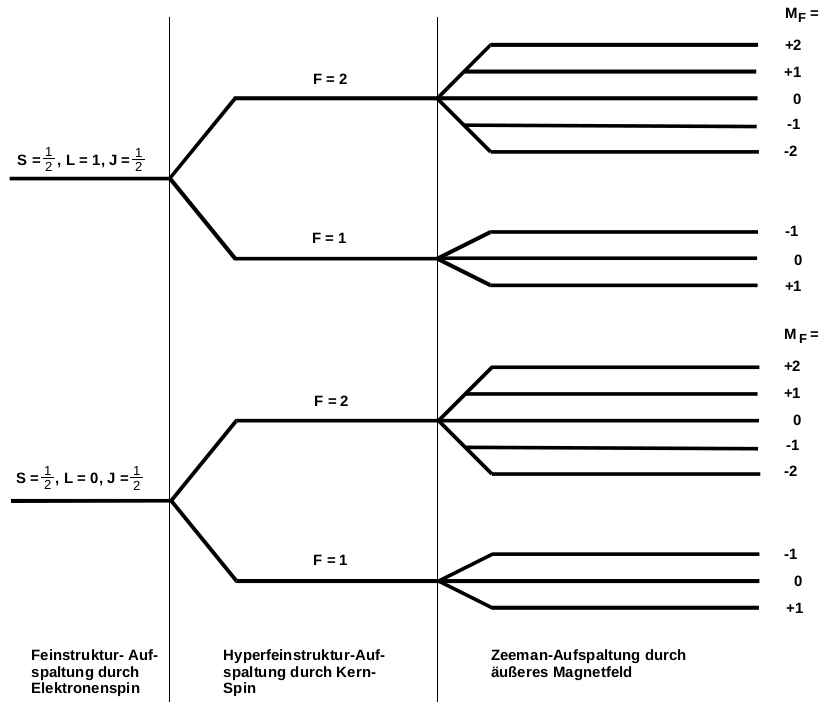
\includegraphics[width=0.8\textwidth]{Hyperfeinstruktur.png}
    \caption{Hyperfeinstruktur und Zeeman-Aufspaltung der Energieniveaus eines Alkali-Atoms mit Kernspin $I=3/2$ \cite[4]{quelle01}.}
    \label{fig:tfig1}
\end{figure}
\FloatBarrier
\noindent
Die aufgespalteten Energieniveaus sind äquidistant mit der Energiedifferenz und Lande-Faktor
\begin{equation}
\Delta E = g_F \mu_B B \qquad g_F \approx g_J \frac{3 F(F+1)+I(I+1)- I(I+1)}{2F(F+2)}\, .
\end{equation}

\subsubsection*{Der Quadratische Zeeman-Effekt}
Für starke Magnetfelder muss der Energiedifferenz \eqref{eq:deltaE} ein Korrekturterm der Form
\begin{equation}
\Delta E = g_F \mu_B B + g_F^2 \mu_B^2 B^2 \frac{1-2M_F}{\Delta E_{Hy}}
\end{equation}
hinzugefügt werden.
$\Delta E_{Hy}$ ist hierbei die Hyperfeinstrukturaufspaltung.
Durch die Abhängigkeit von $M_F$ sind die Energieniveaus des quadratischen Zeeman-Effekts nicht mehr äquidistant.

\subsection{Optisches Pumpen}
Zwischen den Energieniveaus kann es zu verschiedenen Arten von Übergängen kommen, welche in Abbildung \ref{fig:tfig2} dargestellt sind.
Durch spontane und stimulierte Emission gelangt ein Elektron in ein niedrigeres Energieniveau.
Zu stimulierter Emission kann es nur kommen, wenn die Energie $h \nu$ des eintreffende Photons genau der Energiedifferenz der Energieniveaus entspricht.
Absorption tritt auf, wenn die Energie eines eintreffenden Photons ausreicht um ein Elektron auf ein höhergelegendes Energieniveau zu befördern.
\FloatBarrier
\begin{figure}[h]
    \centering
    \includegraphics[width=0.7\textwidth]{übergang.png}
    \caption{Schematische Darstellung der spontanen und induzierten Emission sowie der Absorption \cite{quelle02}.}
    \label{fig:tfig2}
\end{figure}
\FloatBarrier
\noindent

Die Übergänge unterliegen bestimmten Auswahlkriterien, sodass ein Übergang zwischen zwei Energieniveaus nur dann möglich ist, wenn $\Delta M_J$ bestimmen Werten entspricht.
Außerdem können diese Übergänge nur durch Licht einer bestimmten Polarisiation stimuliert werden und bei einer Emission wird auch nur Licht der entsprechenden Polarisiation emittiert.
Es sind drei Arten von Übergängen möglich:
\begin{itemize}
\item \textbf{$\sigma^+$-Übergang}: $\Delta M_J=1$ $\rightarrow$ rechtszirkular polarisiertes Licht
\item \textbf{$\pi$-Übergang}: $\Delta M_J=0$ $\rightarrow$ linear polarisiertes Licht
\item \textbf{$\sigma^+$-Übergang}: $\Delta M_J=-1$ $\rightarrow$ linkszirkular polarisiertes Licht
\end{itemize}
In Abbildung \ref{fig:tfig3} sind die möglichen Übergänge zwischen den Zeeman-Niveaus dargestellt.
\FloatBarrier
\begin{figure}[h]
    \centering
    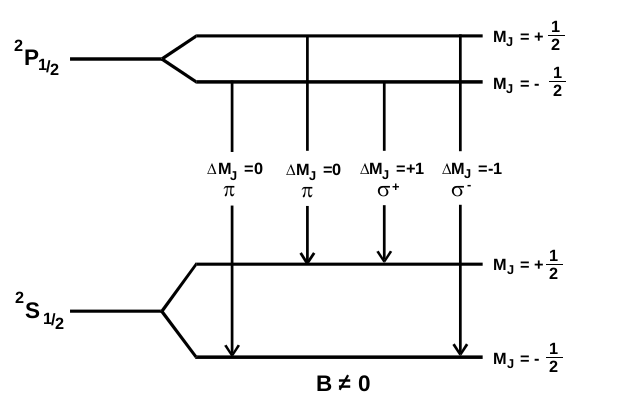
\includegraphics[width=0.8\textwidth]{pumpenschema.png}
    \caption{Mögliche Übergänge zwischen den Zeeman-Niveaus eines Alkali-Atoms ohne Berücksichtigung des Kernspins \cite{quelle01}.}
    \label{fig:tfig3}
\end{figure}
\FloatBarrier
\noindent

Diese selektiven Eigenschaften werden beim optischen Pumpen ausgenutzt, um ein Energieniveau vollständig leerzupumpen.
Hierzu wird ein Dampf bestehend aus Alkali-Atomen in ein Magnetfeld gebracht und mit rechtzirkular polarisierten Licht bestrahlt.
Dieser Dampf befinde sich im thermischen Gleichgewicht, sodass die Atome sich im Grundzustand $^2S_{1/2}$ befinden.
Der Zustand $M_J = -\frac{1}{2}$ ist nach \eqref{eq:boltzmann} aufgrund der geringeren Energie stärker besetzt.
Durch das einstrahlende Licht, welches genau der Energiedifferenz ($D_1$) entspricht, werden die Atome zu einem $\sigma^{+}$-Übergang angeregt und gelangen somit in das $^2P_{1/2}$ Niveau mit $M_J=\frac{1}{2}$.
Von dort aus fallen sie durch spontane Emission zurück in das $^2S_{1/2}$-Niveau, gleichermaßen in das mit der Quantenzahl $M_J = \frac{1}{2}$ und das mit $M_J=-\frac{1}{2}$.
Mit diesem Prozess werden die Atome also von dem $^2S_{1/2}$-Niveau mit $M_J=-\frac{1}{2}$ in das mit $M_J=\frac{1}{2}$ gepumpt und eine Besetzungsinversion erreicht.
Das Pumpverfahren ist in Abbildung \ref{fig:tfig4} dargestellt.
\FloatBarrier
\begin{figure}[h]
    \centering
    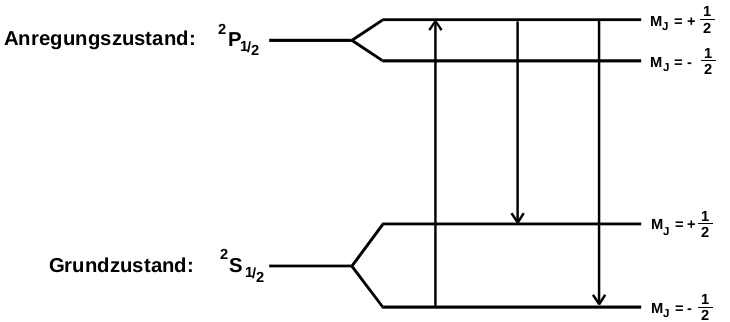
\includegraphics[width=0.7\textwidth]{pumpen.png}
    \caption{Pumpvorgang in einem Alkali-Atom ohne Berücksichtigung der Hyperfeinstruktur \cite{quelle01}.}
    \label{fig:tfig4}
\end{figure}
\FloatBarrier
\noindent
Sobald das $^2S_{1/2}$-Niveau mit $M_J=-\frac{1}{2}$ leergepumpt ist, findet keine Absorption mehr statt und das Gas wird für das rechtzirkulare Licht durchsichtig.
Die Intensität des transmittierten Lichtes zeigt demnach einen, wie in Abbildung \ref{fig:tfig5} dargestellten, Verlauf.
\FloatBarrier
\begin{figure}[h]
    \centering
    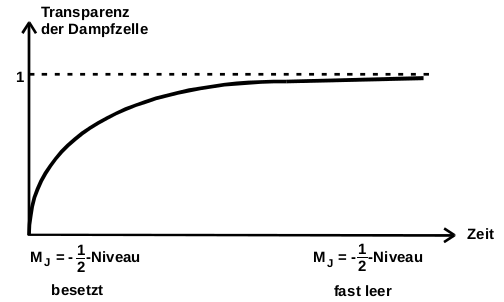
\includegraphics[width=0.6\textwidth]{transmission.png}
    \caption{Verlauf des Transmissionskoeffizienten $T$ in Abhängigkeit der Dauer der Bestrahlung \cite{quelle01}.}
    \label{fig:tfig5}
\end{figure}
\FloatBarrier
\noindent

\subsubsection*{Präzessionsmessung der Zeeman-Aufspaltung}
In diesem Versuch soll das Optische Pumpen genutzt werden um die Energiedifferenz der Zeeman-Niveaus zu bestimmen und somit den Lande-Faktor zu erhalten.
Die Wahrscheinlichkeit für spontane Emission zeigt eine kubische Abhängigkeit von der Frequenz.
Da die Zeeman Niveaus in einem vergleichsweise schmalen Frequenzbereich liegen, spielt spontane Emission kaum eine Rolle und es kann angenommen werden, dass es zwischen den $^2S_{1/2}$-Niveaus nur zu stimulierter Emission kommen kann.
Durch stimulierte Emission können also erneut Atome in das leergepumpte Niveau gelangen. 
Dies ist allerdings nur möglich, wenn das Gas mit einem Hochfrequenzfeld bestrahlt wird, welches genau der Energiedifferenz der Zeeman-Niveaus entspricht
\begin{equation}\label{eq: Magnetfeld}
h\nu = g_J \mu_B B_m \Delta M_J \, .
\end{equation}

Unter Variation des Magnetfeldes, kann beobachtet werden, dass die Absorption wieder einsetzt sobald Gleichung \eqref{eq: Magnetfeld} erfüllt ist.
Denn dann befinden sich wieder Atome im $M_J= -\frac{1}{2}$ Niveau die durch Absorption angeregt werden können.
Der Transmissionskoeffient zeigt also ein Minimum bei $B=B_m$, wie in Abbildung \ref{fig:tfig6} zu sehen ist.
\FloatBarrier
\begin{figure}[h]
    \centering
    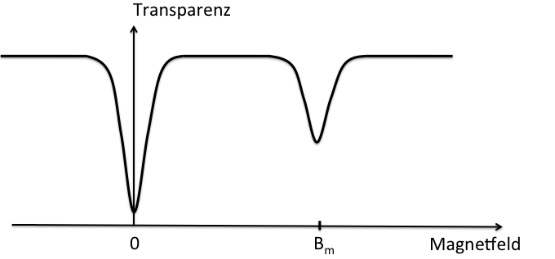
\includegraphics[width=0.6\textwidth]{transmission2.png}
    \caption{Verlauf des Transmissionskoeffizienten $T$ in Abhängigkeit des Magnetfeldes, sowie die erste Resonanz \cite{quelle01}.}
    \label{fig:tfig6}
\end{figure}
\FloatBarrier
\noindent

In Abbildung \ref{fig:tfig6} ist ein weiteres Minimum bei $B=0$ zu sehen.
Dieses kommt dadurch zu stande, dass für B=0 keine Zeeman-Niveaus vorliegen und der optische Pumpprozess somit nicht möglich ist.
Im Realfall wird dieses Minimum nicht genau dann erreicht, wenn das Magnetfeld der Apparatur abgeschaltet ist, sondern dann, wenn dieses das Erdmagnetfeld vollständig kompensiert hat.

Die Magnetfelder in diesem Versuch werden durch Helmholtzspulen erzeugt.
Die magnetische Feldstärke ist zwischen den Spulen näherungsweise konstant und beträgt
\begin{equation}
B= \left(\frac{4}{5}\right)^{\frac{3}{2}}\frac{\mu_0 n I}{R} \, .
\end{equation}

\section{Versuchsaufbau}
\FloatBarrier
\begin{figure}[h]
    \centering
    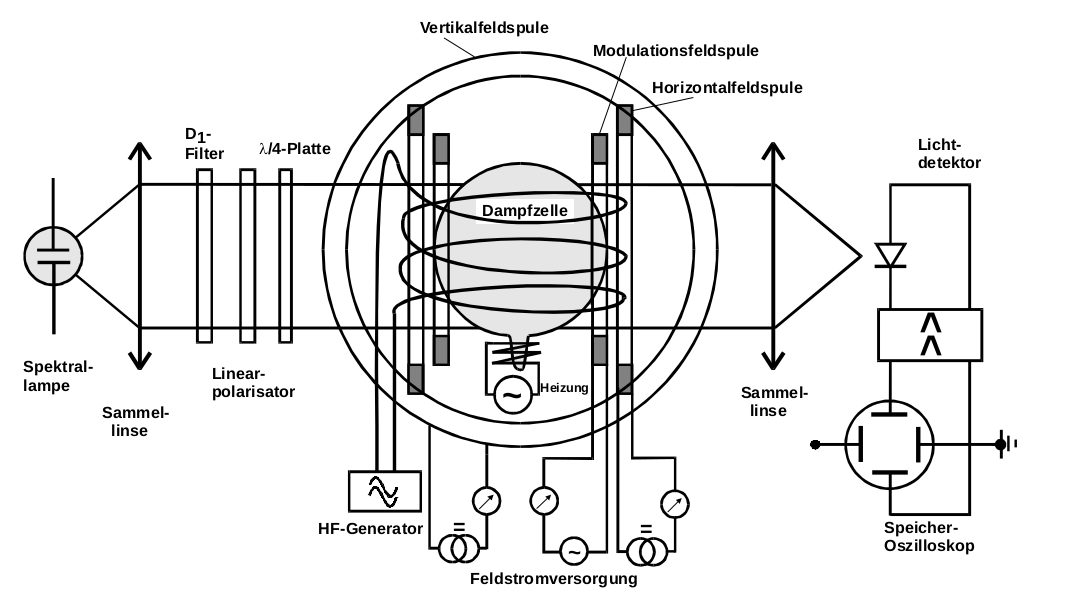
\includegraphics[width=0.8\textwidth]{aufbau.png}
    \caption{Versuchsaufbau des Experiments von oben \cite{quelle01}.}
    \label{fig:tfig7}
\end{figure}
\FloatBarrier
\noindent
Der Aufbau der in diesem Versuch verwendeten Apparatur ist in Abbildung \ref{fig:tfig7} zu sehen.
Das Licht welches die Rubidium Atome anregen soll wird durch eine Rubidium Spektrallampe erzeugt und mit einer Sammellinse kollimiert.
Direkt im Anschluss befinden sich ein Interferenzfilter, ein Polarisationsfilter und ein $\lambda/4$-Plättchen.
Der Intereferenzfilter lässt nur die $D_1$-Wellenlänge ($\lambda = 794,8 \, \si{\nm}$) hindurch, welche benötigt wird um den $\sigma^{+}$-Übergang anzuregen.
Durch den Interferenzfilter wird das Licht zunächst linear polarisiert und durch das $\lambda/4$-Plättchen anschließend das gewünschte rechtszirkular polarisierte Licht erhalten.

In der Dampfzelle befindet sich das Rubidium.
Durch einen Ofen wird diese geheizt um einen optimalen Dampfdruck zu erzeugen.
Das hindurchtretene Licht wird wiederum mit einer Sammellinse auf ein Fotoelement fokussiert, sodass die Lichtintensität von einem Oszilloskop abgelesen werden kann.

Die Dampfzelle ist von drei Helmholtzspulenpaaren umgeben, von denen zwei ein horizonteles Feld und eine ein vertikales Feld erzeugen.
Eine Übersicht der Spulen, deren Eigenschaften und Aufgaben sind in Tabelle \ref{tab:ttab1} zu finden.
\FloatBarrier
\begin{table}[h]
    \centering
    \caption{Eigenschaften der Helmholtzspulenpaare der Apparatur}
    \label{tab:ttab1}
    \begin{tabular}{l l l c l}
        \toprule
        {Spule} & {Ausrichtung} & {Radius} & {Windungen} & {Aufgabe} \\
        \midrule
        Sweep-Spule & horizontal & $16,39\,\si{\cm}$ & $11$ & variierendes Magnetfeld\\
        Horizontalfeld-Spule & horizontal & $15,79\,\si{\cm}$ & $154$ & statisches Magnetfeld\\
        Vertikalfeld-Spule & vertikal & $11,735\,\si{\cm}$ & $20$ & Kompensation des Erdmagnetfeldes\\
        \bottomrule
    \end{tabular}
\end{table}
\FloatBarrier
\noindent


\section{Durchführung}
Bevor mit der Messung begonnen werden kann, werden alle optischen Elemente so justiert, das die maximale Intensität gemessen wird.
Anschließend wird die Apparatur mit einem schwarzen Tuch abgedeckt, damit kein zusätzliches Licht von der Photodiode vernommen wird.
Die Sweep-Spule erzeugt nun ein kontinuierliches Feld zwischen $0-1\,\si{\A}$ mit einer Periode von $2\,\si{\s}$.
Auf dem Oszilloskop ist nun ein breiter Peak, wie der erste in Abbildung \ref{fig:tfig6}, zu beobachten.
Das Erdmagnetfeld ist bestmöglich kompensiert, wenn der Peak besonders schmal ist.
Um einen schmalen Peak zu erreichen, wird die Vertikalspule variiert.
Anschließend wird die Apparatur in Nord-Süd-Richtung gedreht, sodass die horizontale Komponente des Erdmagnetfeldes parralell zum Magnetfeld der Horizontalenfeld-Spule ist.

Es wird eine Sinusspannung mit $100\,\si{\kHz}$ und einer Amplitude von $4\,\text{V}_{\text{pp}}$ angelegt.
Die Frequenzen der RF-Spule werden nun in $100\,\si{kHz}$-Schritten zwischen $100\si{\kHz}$ und $1\si{\MHz}$ erhöht.
Es sind nun immer zwei Peaks zu beobachten, welche jeweils den beiden Isotopen $^{87}$RB und $^{85}$RB zuzuordnen sind.
Für beide Rosonanzen wird jeweils das Magnetfeld $B_m$ gemessen.
Bei höheren Frequenzen muss zusätzlich die Horizontalfeld-Spule angelegt werden um das Sweep-Feld auf die benötigten Bereiche zu verschieben.
Die Einstellung der Horizontalfeld-Spule und die Position an der das Sweep-Feld die Resonanz erreicht werden notiert.


\section{Auswertung}

\section{Diskussion} \label{sec: Diskussion}

\nocite{wingate}
\nocite{*}
\printbibliography

\end{document}